\fancyhead[L]{\textbf{\textsf{MỤC 1.2}}\quad Các mô hình toán học: Danh mục các hàm số cơ bản}
\fancyhead[R]{\textbf{\textsf{25}}}

\noindent
\begin{minipage}[t]{0.26\textwidth}
    \vspace{9.68cm}
    \begin{center}
        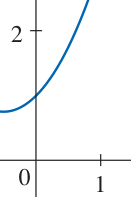
\includegraphics[width=\linewidth]{images/p0060_fig1.png}
        
        \vspace{2pt}
        {\footnotesize (a) $y = x^2 + x + 1$}
        
        \vspace{12pt}
        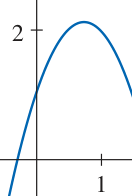
\includegraphics[width=\linewidth]{images/p0060_fig2.png}
        
        \vspace{2pt}
        {\footnotesize (b) $y = -2x^2 + 3x + 1$}
    \end{center}
    
    \vspace{4pt}
    {\footnotesize \textbf{\textsf{HÌNH 7}}\newline
    Đồ thị của các hàm bậc hai là các đường parabol.}
\end{minipage}%
\hfill
\begin{minipage}[t]{0.71\textwidth}
    \noindent\textbf{\textsf{\color{stewartcyan}VÍ DỤ 3}}\quad Sử dụng mô hình tuyến tính cho bởi Phương trình 2 để ước tính nồng độ $\text{CO}_2$ trung bình cho năm 1987 và dự đoán nồng độ cho năm 2025. Theo mô hình này, khi nào nồng độ $\text{CO}_2$ sẽ vượt quá 440 phần triệu (ppm)?

    \vspace{0.25cm}
    \noindent\textbf{\textsf{\color{stewartcyan}LỜI GIẢI}}\quad Sử dụng Phương trình 2 với $t = 1987$, ta ước tính nồng độ $\text{CO}_2$ trung bình vào năm 1987 là
    \[
    C(1987) = 1{,}78242(1987) - 3192{,}90 \approx 348{,}77
    \]
    Đây là một ví dụ về \textit{nội suy} (interpolation) vì chúng ta đã ước tính một giá trị \textit{nằm giữa} các giá trị quan sát được. (Trên thực tế, Đài quan sát Mauna Loa đã báo cáo nồng độ $\text{CO}_2$ trung bình vào năm 1987 là $348{,}93\text{ ppm}$, vì vậy ước tính của chúng ta khá chính xác.)

    Với $t = 2025$, ta được
    \[
    C(2025) = 1{,}78242(2025) - 3192{,}90 \approx 416{,}50
    \]
    Như vậy, ta dự đoán nồng độ $\text{CO}_2$ trung bình vào năm 2025 sẽ là $416{,}5\text{ ppm}$. Đây là một ví dụ về \textit{ngoại suy} (extrapolation) vì chúng ta đã dự đoán một giá trị \textit{nằm ngoài} khoảng thời gian quan sát. Do đó, chúng ta kém chắc chắn hơn nhiều về độ chính xác của dự đoán này.

    Sử dụng Phương trình 2, ta thấy nồng độ $\text{CO}_2$ vượt quá $440\text{ ppm}$ khi
    \[
    1{,}78242t - 3192{,}90 > 440
    \]
    Giải bất phương trình này, ta được
    \[
    t > \frac{3632{,}9}{1{,}78242} \approx 2038{,}18
    \]
    Vì vậy, chúng ta dự đoán nồng độ $\text{CO}_2$ sẽ vượt quá $440\text{ ppm}$ vào năm 2038. Dự đoán này có phần rủi ro vì nó liên quan đến một mốc thời gian khá xa so với các quan sát của chúng ta. Trên thực tế, từ Hình 6 ta thấy xu hướng nồng độ $\text{CO}_2$ tăng nhanh hơn đáng kể trong những năm gần đây, do đó nồng độ này có thể vượt quá $440\text{ ppm}$ từ rất lâu trước năm 2038.
    \hfill{\color{stewartcyan}$\blacksquare$}

    \vspace{0.49cm}
    \noindent{\color{stewartcyan}\rule{1.2ex}{1.2ex}}\hspace{0.5em}\textbf{\textsf{\Large Đa thức}}

    \vspace{0.16cm}
    \noindent Một hàm số $P$ được gọi là một \textbf{đa thức} nếu
    \[
    P(x) = a_n x^n + a_{n-1} x^{n-1} + \dots + a_2 x^2 + a_1 x + a_0
    \]
    trong đó $n$ là một số nguyên không âm và các số $a_0, a_1, a_2, \dots, a_n$ là các hằng số được gọi là các \textbf{hệ số} của đa thức. Tập xác định của mọi đa thức là $\mathbb{R} = (-\infty, \infty)$. Nếu \textbf{hệ số cao nhất} $a_n \neq 0$, thì \textbf{bậc} của đa thức là $n$. Chẳng hạn, hàm số
    \[
    P(x) = 2x^6 - x^4 + \frac{2}{5}x^3 + \sqrt{2}
    \]
    là một đa thức bậc 6.

    Đa thức bậc 1 có dạng $P(x) = mx + b$ và do đó nó là một hàm tuyến tính. Đa thức bậc 2 có dạng $P(x) = ax^2 + bx + c$ và được gọi là một \textbf{hàm bậc hai}. Đồ thị của nó luôn là một parabol nhận được bằng cách tịnh tiến parabol $y = ax^2$, như chúng ta sẽ thấy trong Mục 1.3. Parabol quay bề lõm lên trên nếu $a > 0$ và quay bề lõm xuống dưới nếu $a < 0$. (Xem Hình 7.)

    Đa thức bậc 3 có dạng
    \[
    P(x) = ax^3 + bx^2 + cx + d \qquad a \neq 0
    \]
\end{minipage}